\section{Characterization}
\begin{table}[ht]
    \centering
    \begin{tabular}{l|lll}
         Group & $\text{t}_\text{{max}} [\text{ns}]	$ & $\text{P}_\text{avg} [\text{mW}]$ & $\text{r} [\%] $ \\ \hline \hline
        Philipp, Benedikt &	5,44	& 88,00	& 6,60 \\
        Kratzmann &	5,03 &	185,00 & 13,12 \\
        Essbüchl Jakob &	37,62 &	140	& 1,36 \\
        Glinserer Andreas &	5,89 &	110	& 1,54 \\ 
        Hauk Raphael &	8,08 &	111 &	3,9 \\
        Philipp W. &	2,557 &	121 &	0,477\\
        \hline
    \end{tabular}
    \caption{table with the values}
    \label{tab:my_label}
\end{table}

\begin{figure}[H]
    \centering
    \resizebox{.4\textwidth}{!}{
        \begin{tikzpicture}[scale=0.04,x = {(0.866cm,0.5cm)}, y={(0cm,1cm)}, z={(0.866cm,-0.5cm)},]
            \draw[thin,->] (0,0,0)     -- (40,0,0) node[right] {$t_{max}$}   node[above left]    {40};
            \draw[thin,->] (0,0,0)     -- (0,220,0) node[above] {$P_{avg}$}   node[left]          {220};
            \draw[thin,->] (0,0,0)     -- (0,0,15) node[right] {$r$}           node[below left]    {15};
            \DrawDataUnmarked{o}{black}{5.89}{110}{1.54} % mine
            % others
            \DrawData{x}{red}{5.44} {88}    {6.6}
            \DrawData{x}{red}{5.03} {185}   {13.12}
            \DrawData{x}{red}{37.62}{140}   {1.36} 
            \DrawData{x}{red}{8.08} {111}   {3.9}
            \DrawData{x}{red}{2.557}{121}   {0.477}

        \end{tikzpicture}
    }
    \caption{visualization of table}
    \label{fig:my_label}
\end{figure}

\section{Implementation}

My implementation is as follows: I have additional registers in front of every
instantiated component. The APB bus then reads and writes into/from these 
registers. Due the lack of documentation I implemented the PREADY signal with
a tristates. It would also be possible to implement this as a wire for each
module on its own.

\subsection{Master CTRL}
The master is amplemented with 2 state machines. 
Every state machine is implemented with 2 processes. 1 process
which handles the outputs and another process which handles
the evaluation of the next state. The state change happens in
a synchronous process.
1 of the state
machines handles the APB Protocol and Data exchange on the line. 
It is built after the state machine (fig.\ref{fig:apb-state}) in the AMBA protocol pdf.

\begin{figure}[ht]
    \centering
    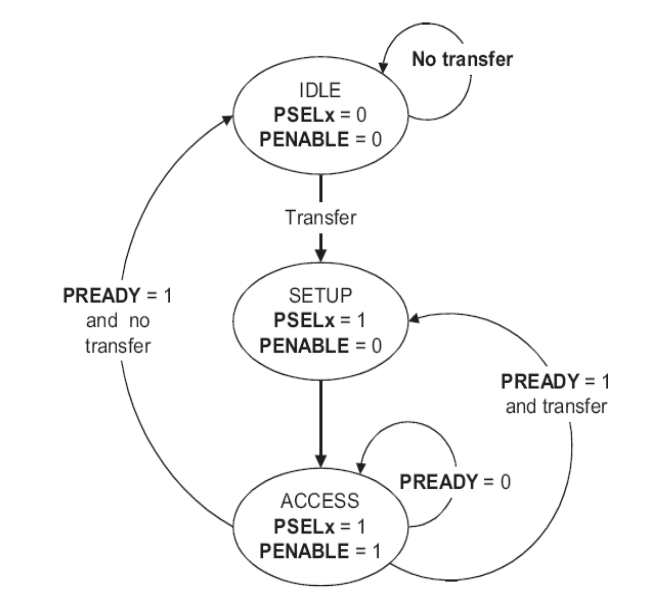
\includegraphics[scale=0.3]{fig/apb-state-diag.png}
    \caption{APB state diagram. Source:\protect\autocite{apb}}
    \label{fig:apb-state}
\end{figure}

The second state machine handles the program procedure (fig.\ref{fig:mst-state}). The 
procedure is as follows: Every $100\,\text{ms}$ it checks if
the switches changed. If a change happened then the new size
gets transmitted to the DSP. Every 
$\dfrac{1}{\text{samples}}\,\text{s}$ it reads the
Sampling part, writes this data then to the DSP, reads the DSP
and then transmits the output from the DSP to the output.

\begin{figure}[ht]
    \centering
    \incfig{master-state-diagram}{1.7}
    \caption{master state diagram. Source: Drawn in Inkscape}
    \label{fig:mst-state}
\end{figure}


\subsection{APB slaves}
The slaves were implemented with the goal to leave the working
parts untouched. This goal was reached by implementing the
slaves as registers. The master writes to the registers and
the slave component reads from the register. Therefore every
slave looks the same with slight modifications:

\lstset{style=vhdl}
\begin{lstlisting}
enable_write <= in_PENABLE and in_PWRITE and in_PSELx;
enable_read  <= not in_PWRITE and in_PSELx;     -- data is read everytime to be ready on the first cycle

out_PREADY <= int_pready;

-- register with the enable sigs as clock
WRITE: process(in_PRESETn, enable_write)
begin
        if in_PRESETn ='1' then
                int_data_write <= x"0000";

        elsif rising_edge(enable_write) then
                int_data_write <= in_PWDATA;
        end if;
end process WRITE;

-- register with the enable sigs as clock
READ: process(in_PRESETn, enable_read)
begin
        if in_PRESETn ='1' then
                out_PRDATA <= x"0000";

        elsif rising_edge(enable_read) then
                out_PRDATA <= int_data_read;

        end if;
end process WRITE;

PREADYP: process(enable_write, enable_read)
begin
        if enable_write='1' or enable_read='1' then
                int_PREADY <= '1';
        else
                int_PREADY <= '0';
        end if;
end process PREADYP;

-- process to forward the data to whatever module or to write into the read register
SFORWARD: process(in_PRESETn, in_PCLK, enable_write, in_PADDR)
begin

        if rising_edge(in_PCLK) then
                if in_PRESETn = '0' then
                        int_data_read <= x"0000";
                else
                        -- here comes handling of signals to write into the read register

                end if; -- rst
        end if; -- rising clock
end process SFORWARD;
\end{lstlisting}

For every slave a new .vhd file was created with the template above in it and an 
instantiation of the component it is the interface to. The ADT slave samples values
and if the CTRL requests values faster it just gets the old value back. If you write
to the DSP part, the DSP holds the bus transmission by holding the PREADY signal low
until the new value is computed.

\subsection{LEDs}
\begin{table}[ht]
    \centering
    \begin{tabular}{|l|l|l|l|l|l|l|l|}
        \hline
         LD15 & LD14 & LD13 & LD12 & LD11 & LD10 & LD09 & LD08 \\ \hline
         \multicolumn{8}{|c|}{Buffer size of the DSP binary encoded} \\ \hline
         \multicolumn{8}{c}{} \\ \hline
         LD07 & LD06 & LD05 & LD04 & LD03 & LD02 & LD01 & LD00 \\ \hline
         ADT & \multicolumn{3}{c|}{CTRL size} & STATE & \multicolumn{3}{c|}{DSP size} \\ \hline
    \end{tabular}
    \caption{LED explanation}
    \label{tab:leds}
\end{table}

\begin{itemize}
    \item ADT - signals everytime the ADT samples a new value
    \item CTRL size - the size saved in CTRL part as power of two. 
        E.g. $\text{b'}1 1 0 = 6 -> 2^6 = 64$ buffer size.
    \item STATE - toggles everytime the CTRL goes into the idle state
    \item DSP size - same as CTRL size but saved in the DSP part
\end{itemize}

\subsection{Simulation}
Here are two images from the simultion. The first one shows the way
the master works in respect to polling the switch slave. The switch
slave select wire is choosen more often. And corresponding to the 
countersize it starts a normal cycle. The normal cycle can be seen in 
the second simulation image.
\newpage

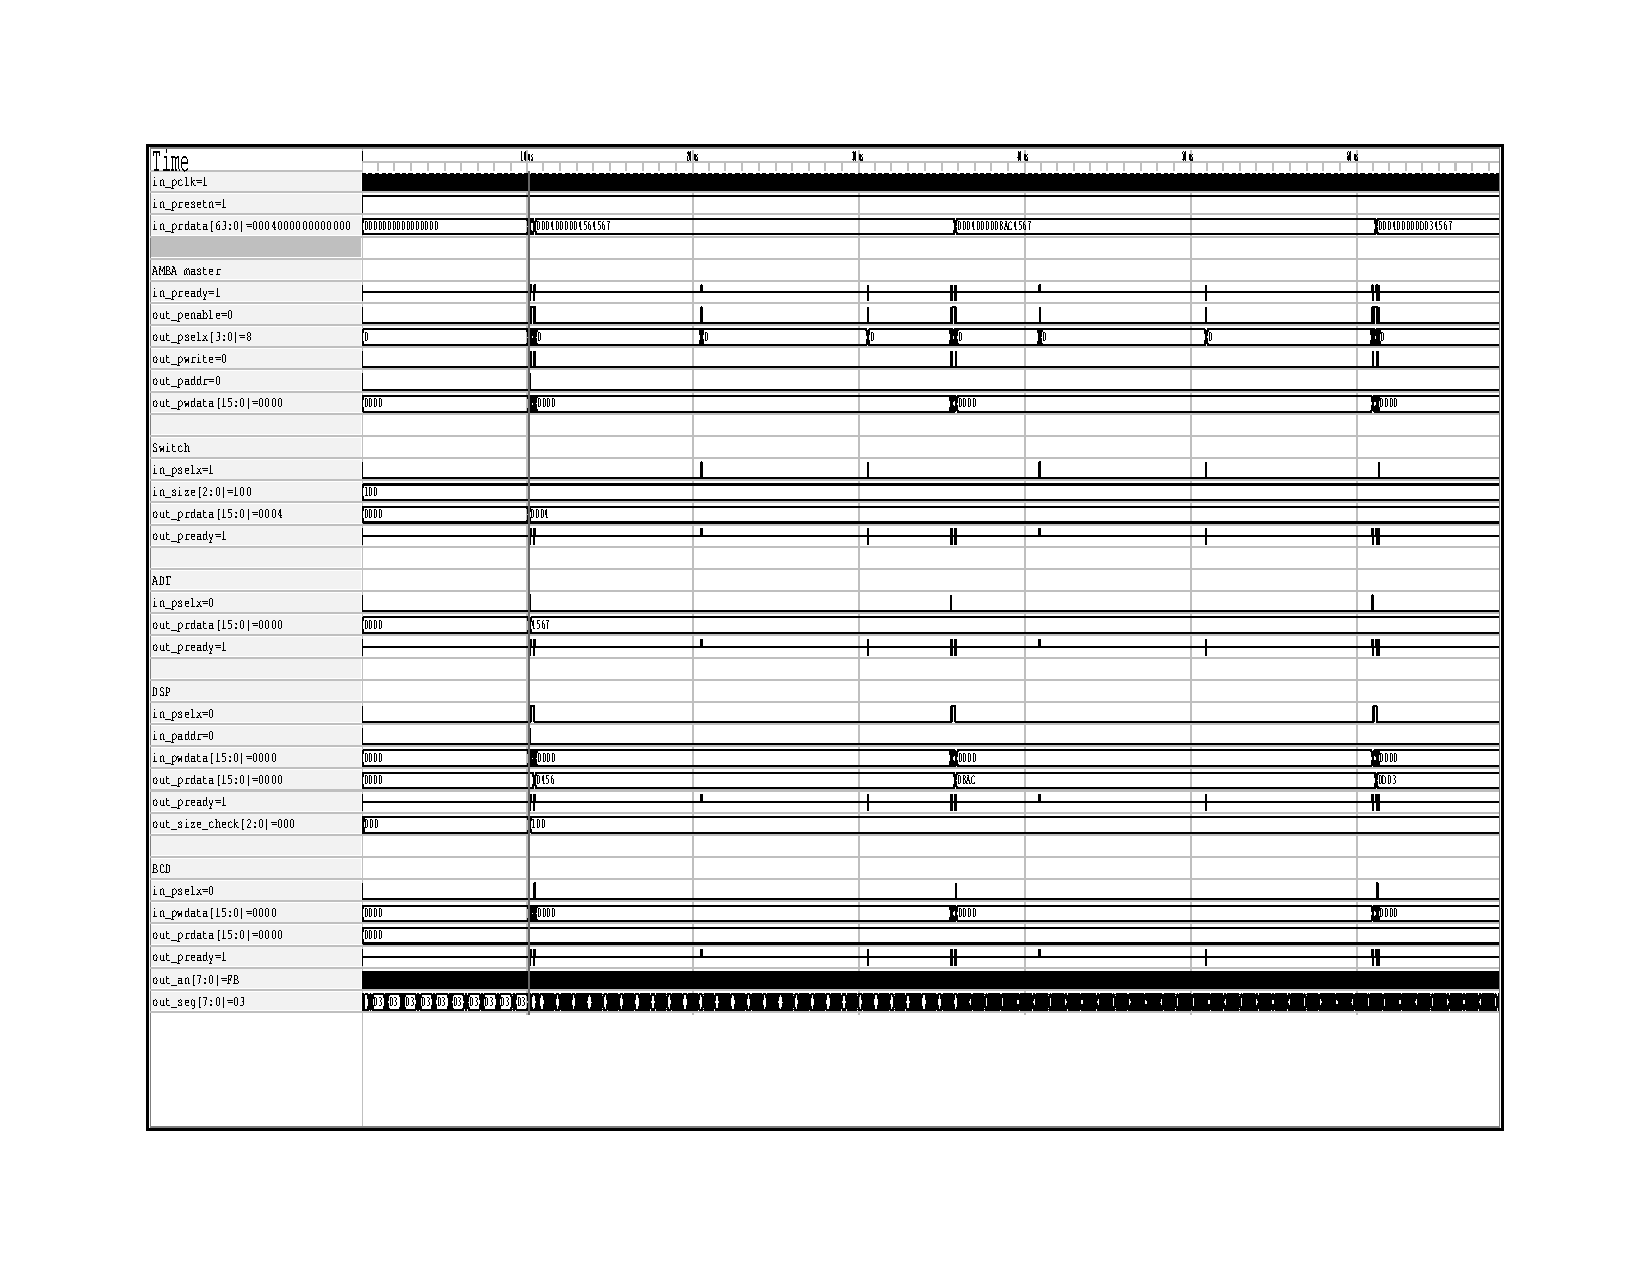
\includepdf[landscape=true,pages=1]{./fig/simulation1.pdf}

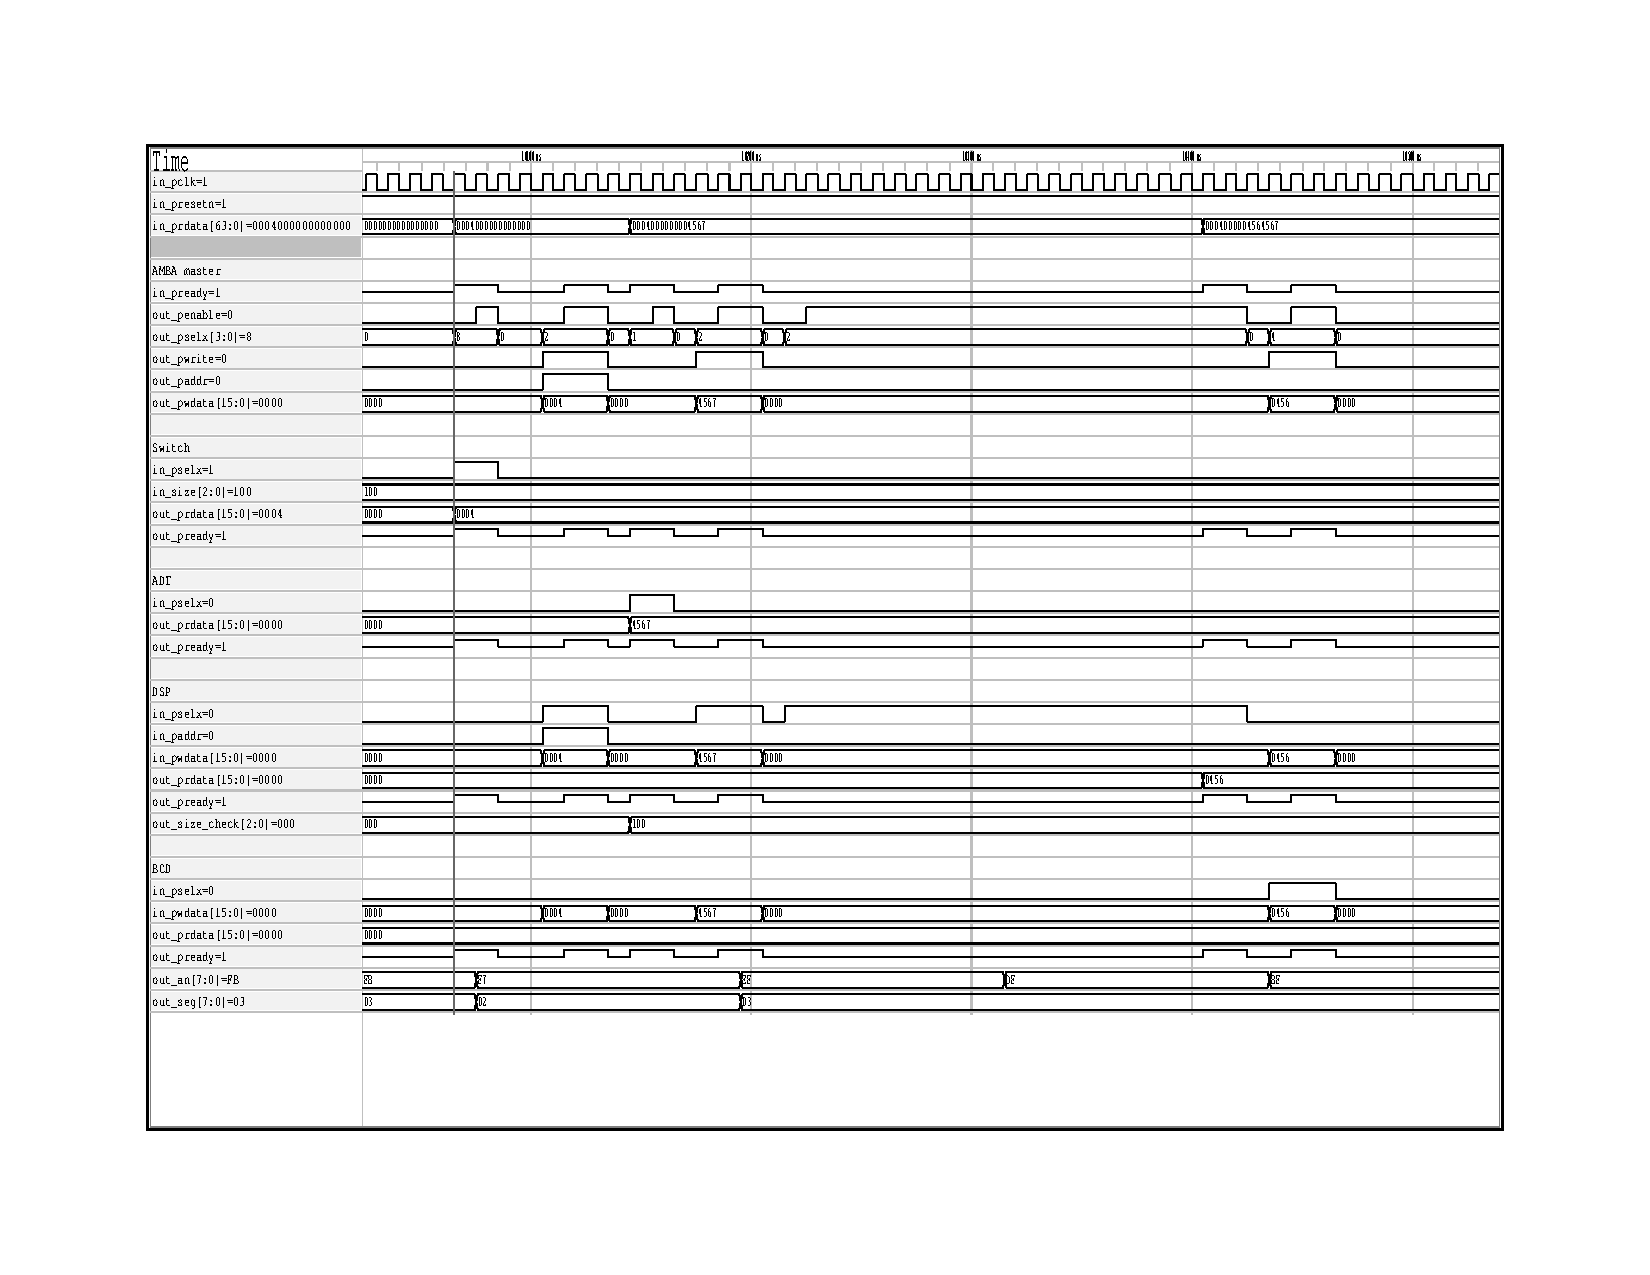
\includepdf[landscape=true,pages=1]{./fig/simulation2.pdf}
\newpage
\subsection{Problems}
I had many problems with my first implementation because I misunderstood a 
central point in the AMBA APB specification. Thanks to this mistake I had
race conditions in my design which caused my simulation to work but my 
implementation to only work sometimes. Much time was wasted by trying it
this way. To clarify my mistake: I tried not to write into registers but
to directly write into the components. By doing it this way I got many
additional conditions to wait for values and multiple sources for enable
signals. Somewhere in between then I got the race condition.

\subsection{Reports}
\subsubsection{utilization report}
\lstinputlisting[basicstyle=\tiny,firstnumber=1]{post_route_utilization.rpt}
\subsubsection{timing report}
In the timing report you can see many pins which are not driven by a clock pin.
This is per design, because APB can react asynchronously to operations. Waiting
for the rising clock edge everytime would always add a wait state.
\lstinputlisting[basicstyle=\tiny,firstnumber=1]{post_route_timing_summary.rpt}
